\section{Gaze control}
\label{Sec:gazecontrol}

One of the main modules in the reaching controller is represented 
by the {\tt gaze controller}, which directs gaze toward a given 
target. The input of this module is represented by the target 
location in the image planes. The output instead consists in the head 
motor commands necessary to direct gaze toward the target. 

\begin{figure}[tbp]
\centering
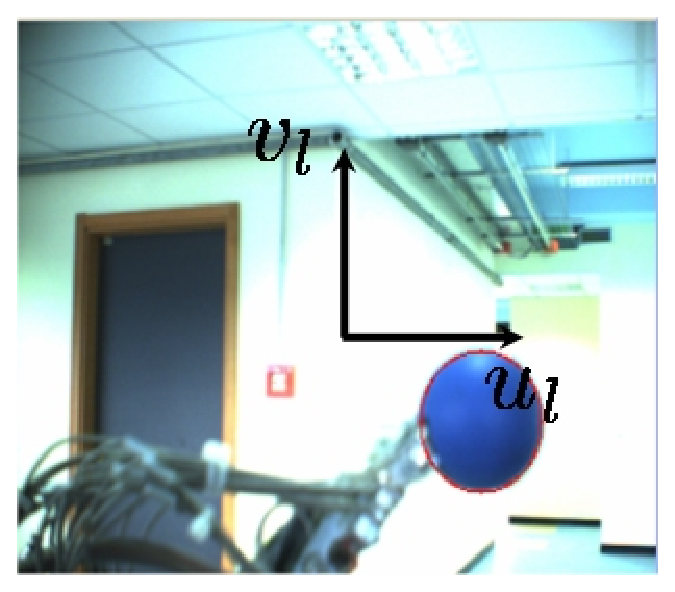
\includegraphics[width=25mm]{Figure/LeftImage.eps} \hspace{1cm}
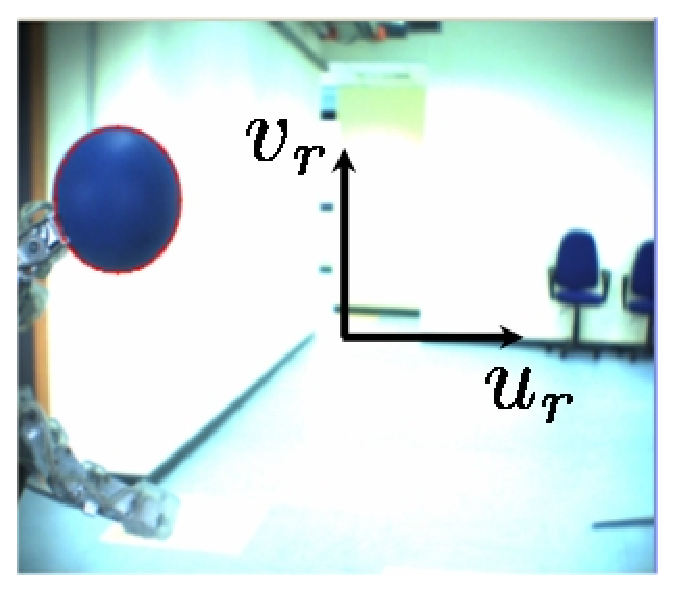
\includegraphics[width=25mm]{Figure/RightImage.eps}
\caption{Two typical images taken from the two cameras mounted on the 
eyes of the robot (resolution 320$\times$240). 
The coordinates of the target (the blue ball) on the image planes
will be denoted $u_r$, $v_r$, and $u_l$, $v_l$ (respectively right 
and left cameras).}
\label{Fig:ImagePlane}
\end{figure}
 
The crucial aspect in this case concerns the redundancy of the 
head. Let $u_r$ and $v_r$ be the coordinates of the target on the 
right image plane. Similarly, let $u_l$ and $v_l$ be the coordinates 
of the target on the 
left image plane (see Figure \ref{Fig:ImagePlane}). The values of $u_r$, 
$v_r$, $u_l$, $v_l$ are the output of a visual model whose description 
is not important in this paper. Directing gaze toward the target 
consists in moving the neck and the eyes so as to obtain 
$u_r=0$, $v_r=0$, $u_l=0$, $v_l=0$. 
Let us define the vector 
$\tilde {\mathbf u}_{target}= \begin{bmatrix} u_r & v_r & u_l & v_l 
\end{bmatrix}^\top \in \mathbb R^4$ corresponding to the 
target location in the image planes. Assuming that the target is stationary 
with respect to the robot, we have that $\tilde {\mathbf u}_{target}$ 
can be expressed as a function of the head configuration 
$\mathbf q_{head} = \begin{bmatrix} \mathbf q_{eyes}^\top & \mathbf q_{neck}^\top \end{bmatrix}^\top \in \mathbb R^6$:
\begin{eqnarray*}
\tilde {\mathbf u}_{target} = \tilde f_{head} (\mathbf q_{head}),
\end{eqnarray*}
where the function $\tilde f_{head} : \mathbb R^6 \longrightarrow \mathbb R^4$ 
depeends on the head kinematics. Under reasonable 
assumptions, we do not need to impose simultaneously 
the four conditions $u_r=0$, $v_r=0$, $u_l=0$, $v_l=0$.  Our control task 
can be redefined as the problem of controlling 
$\utarget = \begin{bmatrix} u_r & u_l & v_l \end{bmatrix}^\top \in \mathbb R^3$ 
to zero. The kinematic function will be in this case:
\begin{eqnarray*}
\utarget = f_{head} (\mathbf q_{head}), \qquad f_{head} : \mathbb R^6 \longrightarrow \mathbb R^3.
\end{eqnarray*}
Clearly, the task specification does not constrain all the head degrees of 
freedom (we are imposing $m=3$ constraints but we have $n=6$ free variables 
available: we remain with $n-m=3$ additional degrees of freedom). 
Practically, we can have 
different configuration of the head ($\mathbf q_{head,1} \neq \mathbf 
q_{head,2}$) both keeping the same target in fixation 
(${\mathbf u}_{target,1} = {\mathbf u}_{target,2} = 0$). 
The strategy we have chosen to solve this ``redundancy problem'' consists in 
using two controller for the eyes and the neck. The former controls 
the eyes version and common tilt to track the object, while the latter
controls neck yaw and pitch to maintain the eyes ``centered'' within 
the neck. Mathematically the above strategy can be implemented 
as follows:

\begin{eqnarray} \label{Eq:HeadEyeControl}
\left\{ \begin{matrix}
\dot {\alpha_v^c} &=&   K_p (u_l + u_r)\\
\dot {\theta_y} &=&   K_y \alpha_v^c \\
\dot {\alpha_t^c} &=&   K_t (v_l + v_r)\\
\dot {\theta_p} &=&   K_r \alpha_t^c
\end{matrix} \right.,
\end{eqnarray}
where $\alpha_t^c$ and $\alpha_v^c$ are the eyes version and common tilt and 
where $\theta_y$ and $\theta_p$ are the yaw and pitch movement of the neck. 
In the proposed control scheme, the vergence degree of freedom $\alpha_v^d$, 
which corresponds to the distance of the target does not influence 
the neck position and is therefore controlled separately from the neck:
\begin{eqnarray} 
\dot {\alpha_v^d} &=&   K_p (u_l - u_r).
\end{eqnarray}
Finally, the neck roll degree of freedom $\theta_r$ is maintained fixed, 
i.e. $\theta_r^d=0$.

The proposed control strategy allows us to asymptotically fixate the target 
($u_l \rightarrow 0$, $v_l \rightarrow 0$, $u_r \rightarrow 0$ which 
implies $v_r \rightarrow 0$) while also also guaranteeing an asymptotically 
straight gaze ($\alpha_v^c \rightarrow 0$, $\alpha_t^c \rightarrow 0$). Moreover
, by choosing a suitable value for the gains $K_p$, $K_y$, $K_t$ and $K_r$ it
is possible to achieve an asymptotic behavior with the eyes moving rapidly on 
the target and the neck following the eye movement with a slower 
movement.
